\chapter{A luz viaja em linha reta}\label{ch:g4:light-straight-lines}

Feixes de sol atravessam inclinados a névoa da manhã entre as árvores
--- retos como barbantes esticados, todos eles. Uma lanterna num
sótão empoeirado joga uma lâmina de \omterm{def:g1:light-and-shadows:source}{luz} de bordas retas. Você
consegue ouvir um colega chamando da esquina, mas não consegue
\emph{vê-lo} lá. Tudo isso é uma única lei vestida com roupas
diferentes --- a lei mais antiga da \omterm{def:g1:light-and-shadows:source}{luz}.

\section{A lei da linha reta}

\begin{proposition}[A luz viaja em linha reta]\label{prop:g4:light-straight-lines:law}
No \omterm{def:g2:air-around-us:air}{ar} (como na água, no vidro ou no espaço vazio), a \omterm{def:g1:light-and-shadows:source}{luz} viaja em
linha reta. Ela não faz curva nas esquinas, não \omterm{def:g1:floating-and-sinking:words}{flutua} à toa como a
fumaça, não se entorta para achar você atrás de uma parede. Onde uma
linha reta partindo da fonte não chega, não chega \omterm{def:g1:light-and-shadows:source}{luz} nenhuma dessa
fonte.
\end{proposition}

\begin{definition}[Raio de luz]\label{def:g4:light-straight-lines:ray}
Para desenhar a \omterm{def:g1:light-and-shadows:source}{luz}, os físicos usam o \emph{raio de luz}\index{raio
de luz}: uma linha reta com uma seta, mostrando um fio de \omterm{def:g1:light-and-shadows:source}{luz} e o
sentido em que ele corre. O feixe de uma lanterna é desenhado como um
leque de raios; um feixe fino de laser, como um raio só. Como a seta
da \omterm{def:g2:pushes-and-pulls:force}{força}, o raio é um desenho pequeno que carrega uma lei dentro
dele: as estradas da \omterm{def:g1:light-and-shadows:source}{luz} são retas como uma régua.
\end{definition}

\begin{omfigure}
\begin{tikzpicture}[scale=0.85]
  \draw[thick, fill=omExo, fill opacity=0.3]
    (0.2,1.3) rectangle (1.4,2.3);
  \draw[thick] (1.4,1.45) -- (1.4,2.15);
  \draw[-Stealth, omThm, thick] (1.4,2.1) -- (10.6,2.9);
  \draw[-Stealth, omThm, thick] (1.4,1.8) -- (10.6,1.8);
  \draw[-Stealth, omThm, thick] (1.4,1.5) -- (10.6,0.7);
  \node[below, font=\small] at (0.8,1.1) {lanterna};
  \node[above, font=\small] at (6.0,2.75)
    {um leque de raios: cada um reto como uma régua};
\end{tikzpicture}

{\small O feixe de uma lanterna desenhado do jeito dos físicos: raios
retos, com setas mostrando para onde a \omterm{def:g1:light-and-shadows:source}{luz} corre.}
\end{omfigure}

\begin{example}[Onde a lei se mostra]\label{ex:g4:light-straight-lines:sightings}
Depois que se conhece a lei, ela aparece em toda parte: os feixes
retos de sol na névoa ou entre as ripas de uma persiana; a borda reta
e nítida do feixe de uma lanterna no \omterm{def:g2:air-around-us:air}{ar} empoeirado; o fio absolutamente
reto de um apontador laser; e todo farol varrendo lâminas retas de
\omterm{def:g1:light-and-shadows:source}{luz} pelo mar noturno. \omterm{def:g1:light-and-shadows:source}{Luz} entortada nunca se vê --- chafarizes e
florestas podem fazer curva, a \omterm{def:g1:light-and-shadows:source}{luz} não faz.
\end{example}

\begin{omfigure}
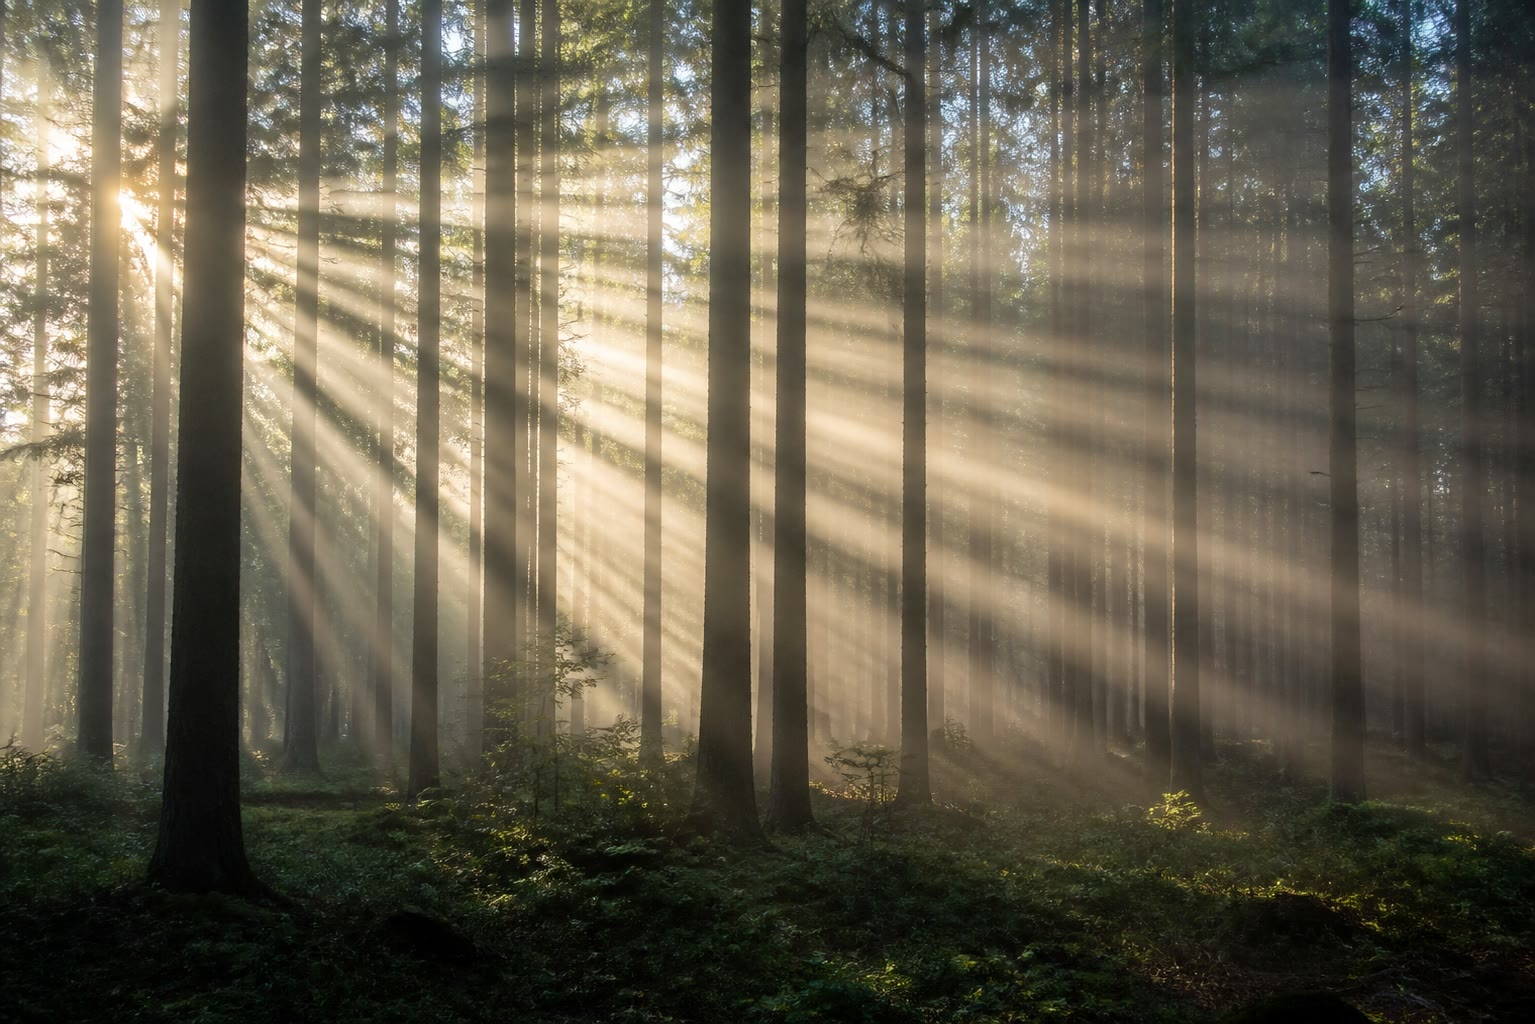
\includegraphics[width=0.58\linewidth]{images/book1/ai/g4-light-sunbeams.jpg}

{\small A prova da própria natureza: os feixes de sol atravessando o \omterm{def:g2:air-around-us:air}{ar} enevoado são perfeitamente retos --- a \omterm{def:g1:light-and-shadows:source}{luz} não faz curva em volta das árvores.}
\end{omfigure}

\section{Provando com três cartões}

\begin{method}[A experiência dos três cartões]\label{met:g4:light-straight-lines:cards}
\begin{enumerate}
  \item Faça um furinho no meio de três cartões rígidos, todos na
        mesma altura;
  \item ponha os cartões em pé, em fila, com um palmo de distância
        entre eles, e uma vela acesa (ou uma lanterna) atrás do
        último;
  \item mexa a cabeça até enxergar a chama através dos três furos ---
        só possível quando os três furos e a chama estiverem numa
        mesma linha reta (confira: um barbante esticado passando
        pelos furos chega à chama);
  \item agora deslize o cartão do meio para o lado, só a largura de
        um dedo.
\end{enumerate}
A chama some. A \omterm{def:g1:light-and-shadows:source}{luz} que poderia ter ziguezagueado --- pelo primeiro
furo, um pulinho para o lado, pelo furo deslocado e daí até o seu
olho --- simplesmente não faz isso: sem linha reta, sem \omterm{def:g1:light-and-shadows:source}{luz}.
\end{method}

\begin{omfigure}
\begin{tikzpicture}[scale=0.85]
  \draw[thick] (1.0,0.3) -- (1.0,2.5) (3.6,0.3) -- (3.6,2.5)
    (6.2,0.3) -- (6.2,2.5);
  \fill[white] (0.92,1.32) rectangle (1.08,1.48);
  \draw[thick] (0.92,1.32) rectangle (1.08,1.48);
  \fill[white] (3.52,1.32) rectangle (3.68,1.48);
  \draw[thick] (3.52,1.32) rectangle (3.68,1.48);
  \fill[white] (6.12,1.32) rectangle (6.28,1.48);
  \draw[thick] (6.12,1.32) rectangle (6.28,1.48);
  % a real candle: wax body, wick, teardrop flame
  \draw[thick, fill=yellow!15] (8.42,0.3) rectangle (8.78,1.02);
  \draw[thick] (8.6,1.02) -- (8.6,1.16);
  \draw[thick, orange!80!red, fill=yellow!80]
    (8.6,1.16) .. controls (8.44,1.3) and (8.47,1.47) .. (8.6,1.58)
    .. controls (8.73,1.47) and (8.76,1.3) .. (8.6,1.16);
  \fill[orange!90] (8.6,1.27) ellipse (0.045 and 0.08);
  % the ray of light, dead straight through the three holes
  \draw[-Stealth, line width=1.3pt, yellow!75!orange]
    (8.44,1.4) -- (-0.4,1.4);
  \node[below, font=\small] at (8.6,0.05) {vela};
  \node[below, font=\small] at (-0.2,1.2) {olho};
  \node[above, font=\small] at (4.6,2.55)
    {três furos numa linha reta: a chama é vista};
\end{tikzpicture}

{\small A experiência dos três cartões: a chama fica visível
exatamente quando chama, furos e olho estão alinhados em linha reta.
Desloque um cartão e a vista morre.}
\end{omfigure}

\begin{example}[As sombras explicadas de vez]\label{ex:g4:light-straight-lines:shadows}
Agora a \omterm{def:g1:light-and-shadows:shadow}{sombra} do seu primeiro ano de escola entrega o segredo dela.
Os raios correm retos a partir da lâmpada; a bola detém os que batem
nela; os raios que passam raspando a borda seguem retos em frente.
Atrás da bola fica exatamente o espaço que nenhum raio reto consegue
alcançar --- a \omterm{def:g1:light-and-shadows:shadow}{sombra}, com a borda nítida desenhada pelos últimos
raios que escaparam. Raios retos, \omterm{def:g1:light-and-shadows:shadow}{sombras} nítidas: uma \omterm{def:g1:light-and-shadows:source}{luz} torta
borraria toda \omterm{def:g1:light-and-shadows:shadow}{sombra} numa névoa.
\end{example}

\section{Enxergar é receber luz}

\begin{proposition}[Como funciona a visão]\label{prop:g4:light-straight-lines:seeing}
Você enxerga uma coisa quando a \omterm{def:g1:light-and-shadows:source}{luz} dela viaja em linha reta até o
seu olho --- a \omterm{def:g1:light-and-shadows:source}{luz} própria dela, se for uma fonte, ou a \omterm{def:g1:light-and-shadows:source}{luz} do Sol ou
da lâmpada que ela devolve, nos outros casos. Nada sai do seu olho
para agarrar o mundo: enxergar é \emph{receber}, pegar raios como uma
rede pega bolas.
\end{proposition}

\begin{example}[Do outro lado da esquina]\label{ex:g4:light-straight-lines:corner}
O seu colega chama da esquina da escola: você o ouve, mas não
consegue vê-lo. O \omterm{def:g3:sound-around-us:sound}{som} se espalha como os anéis num lago e contorna a
quina; a \omterm{def:g1:light-and-shadows:source}{luz} mantém as suas estradas retas, e nenhuma linha reta liga
o rosto do seu colega ao seu olho através do tijolo. Para enxergar
depois de uma esquina, é preciso \emph{dobrar a estrada} --- dar ao
raio uma superfície dura e brilhante em que ele possa quicar. Esse
truque se chama espelho, e ele é o dono do primeiro capítulo de \omterm{def:g1:light-and-shadows:source}{luz}
do ano que vem.
\end{example}

\begin{remark}[O corredor campeão]\label{rem:g4:light-straight-lines:speed}
O \omterm{def:g3:sound-around-us:sound}{som}, como medimos, trota a \qty{340}{m} por segundo. A \omterm{def:g1:light-and-shadows:source}{luz}, nas
estradas retas dela, joga em outra liga: ela atravessa o céu inteiro
mais depressa do que qualquer contagem consegue acompanhar --- e é
por isso que o clarão chega ``na hora'' e o trovão se arrasta alguns
segundos atrás. E quão rápido, exatamente? O número é tão absurdo que
o guardamos para um ano mais adiante --- junto com a história dos
truques espertos que foram necessários para medi-lo.
\end{remark}

\section{Exercícios}

\begin{exercise}[$\star$]\label{exo:g4:light-straight-lines:1}
Enuncie a lei deste capítulo. Diga dois lugares ao \omterm{def:g2:air-around-us:air}{ar} livre em que
ela pode ser vista.
\end{exercise}

\begin{exercise}[$\star$]\label{exo:g4:light-straight-lines:2}
O que é um \omterm{def:g4:light-straight-lines:ray}{raio de luz}, e quais duas coisas o desenho dele mostra?
\end{exercise}

\begin{exercise}[$\star$]\label{exo:g4:light-straight-lines:3}
Na experiência dos três cartões, em que caso exatamente você
consegue ver a chama? Qual movimento único a faz sumir, e por quê?
\end{exercise}

\begin{exercise}[$\star$]\label{exo:g4:light-straight-lines:4}
Como a lei da linha reta explica a borda nítida de uma \omterm{def:g1:light-and-shadows:shadow}{sombra}?
\end{exercise}

\begin{exercise}[$\star$]\label{exo:g4:light-straight-lines:5}
Você está vendo este livro agora. Conte a viagem da \omterm{def:g1:light-and-shadows:source}{luz} que torna
isso possível, de uma lâmpada até o seu olho.
\end{exercise}

\begin{exercise}[$\star$]\label{exo:g4:light-straight-lines:6}
Por que você consegue ouvir um colega do outro lado da esquina mas
não consegue vê-lo? O que cada viajante --- o \omterm{def:g3:sound-around-us:sound}{som} e a \omterm{def:g1:light-and-shadows:source}{luz} --- faz na
esquina?
\end{exercise}

\begin{exercise}[$\star$]\label{exo:g4:light-straight-lines:7}
Um buraco de fechadura, um cômodo iluminado do outro lado e o seu
olho: de que pontos do corredor escuro dá para ver a lâmpada pelo
buraco da fechadura? Responda com uma linha reta.
\end{exercise}

\begin{exercise}[$\star$]\label{exo:g4:light-straight-lines:8}
De um fogo de artifício distante, o que chega primeiro: o estouro ou
o clarão? Qual lei e qual medida deste ano explicam a diferença?
\end{exercise}

\begin{exercise}[$\star$]\label{exo:g4:light-straight-lines:9}
``Quando eu olho para uma \omterm{def:g4:solar-system:star}{estrela}, alguma coisa sai do meu olho para
tocar nela.'' Corrija essa crença antiga com a
\cref{prop:g4:light-straight-lines:seeing} --- o que viaja, e em que
sentido?
\end{exercise}

\begin{exercise}[$\star\star$]\label{exo:g4:light-straight-lines:10}
Projete, com um desenho de raios, um jeito de observar o corredor de
dentro do seu quarto usando o truque do espelho anunciado no
\cref{ex:g4:light-straight-lines:corner}: onde a superfície
brilhante precisa ficar, na porta, e o que ela faz com a estrada do
raio? (Os submarinos usam exatamente isso, empilhado duas vezes, para
enxergar acima das ondas.)
\end{exercise}

\begin{exercise}[$\star\star$]\label{exo:g4:light-straight-lines:11}
Numa manhã de névoa, os feixes de sol se abrem em leque entre as
árvores em linhas visivelmente retas --- e o seu colega diz: ``A
gente vê os feixes, então a \omterm{def:g1:light-and-shadows:source}{luz} deve ser um material visível
pendurado no \omterm{def:g2:air-around-us:air}{ar}.'' O que vocês dois estão realmente vendo quando um
``feixe'' aparece na névoa ou na poeira, e como esse feixe ficaria num
\omterm{def:g2:air-around-us:air}{ar} perfeitamente limpo?
\end{exercise}
